%!TEX root = ../../csuthesis_main.tex
\chapter{考虑边缘计算的无人机航迹规划及任务调度算法}

\section{算法设计应用流程}

\begin{figure}[!htbp]
    \centering
    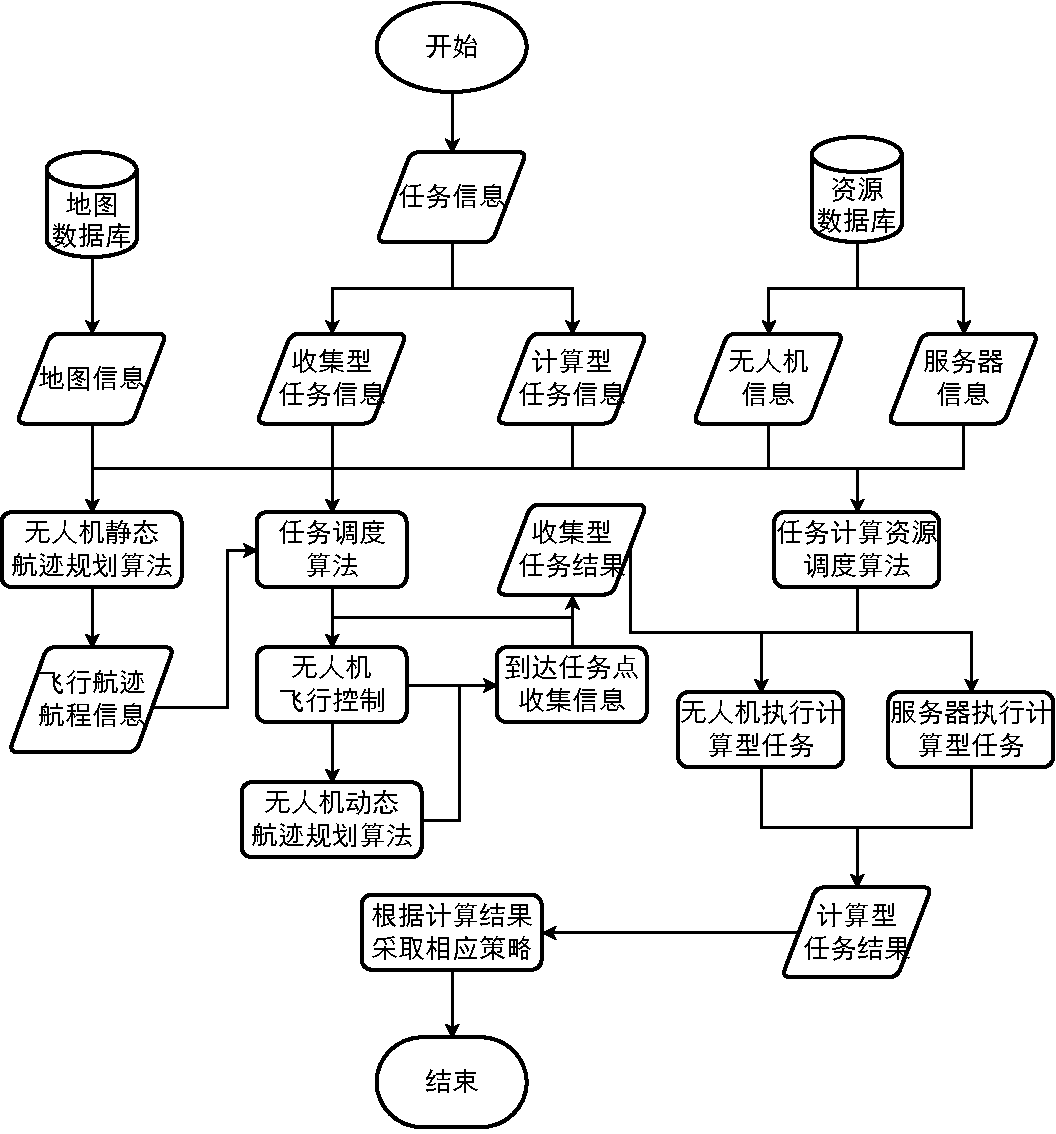
\includegraphics[width=0.9\textwidth]{images/算法设计应用流程.pdf}
    \caption{算法设计应用流程}
    \label{fig:算法设计应用流程}
\end{figure}

本文针对无人机航迹规划及任务调度问题所设计的算法的应用流程如下,首先将所给的任务信息分解成收集型任务信息和计算型任务信息,然后服务器根据收集型任务信息、从资源数据库中得到的无人机信息、从地图数据库中得到的地图信息,放入静态场景下的无人机航迹规划算法中,得到各点间的无人机飞行航迹和航程的对应信息,再将以上信息以及收集型任务信息放入任务调度算法,得到所需无人机的数量、每个无人机需要执行的收集型任务有序序列、无人机飞行航迹等信息;同时服务器再根据计算型任务信息、无人机信息和服务器信息通过任务计算资源调度算法,为每一个计算型任务分配对应的计算设备;然后无人机根据所给的任务序列和飞行航迹进行飞行控制,若遇到航迹中的存在的障碍物则使用动态场景下的航迹规划算法修订航迹来回避障碍物,在到达任务点后执行收集型任务,在完成后将收集得到的任务结果传输至执行该收集型任务对应的计算型任务的设备中进行计算,在计算型任务完成后,便能够根据任务结果采取相应的措施,流程如图~\ref{fig:算法设计应用流程}所示。

\section{面向边缘计算的任务计算资源调度算法}

由于生成任务计算资源调度方案需要无人机的航程信息,而在无人机飞行过程中,随时可能因为出现与原定航迹相冲突的障碍物而对航迹进行修订,进而使其航程信息发生变化,因此在解决该问题时,本文先将该问题分为无人机尚未接收到指令开始执行任务前的静态场景以及无人机开始执行任务,但由于中途进行了避障操作而使得原本的资源调度方案需要重新生成的动态场景。在静态场景中,由于不需要在很短时间内给出调度方案,因而计算资源调度方案的质量比算法计算时间更为重要;而在动态场景中,由于场景信息不断发生变动,为避免计算资源调度方案的生成时间过长导致无人机的数据传输需要进行等待,进而导致系统效率下降,此时算法的运行时间更为重要。

基于以上分析,本文提出的面向边缘计算的任务计算资源调度算法共包含两个算法,分别是用于求解静态场景的参数自适应的模拟退火算法(Adaptive Simulated Annealing, ASA)以及用于求解动态场景的快速决策算法(Fast Decision-making Algorithm, FD)。

\subsection{基于ASA的静态场景下的任务计算资源调度算法}

本算法是在传统SA算法的基础上,对其进行了邻域结构以及参数方面的改进。

\subsubsection{邻域结构设计} \label{sec:neighbor_design}

由于需要执行的任务数是一定的,且一个任务仅由一个设备进行处理计算,而一个设备可能需要处理多个任务,因此可以简单地使用一个数组来作为算法的解,其中数组的元素对应的位置为任务的序号、数组的元素为设备的序号,以此来设计本文所使用的邻域结构。

第一种邻域结构为任务交换邻域结构,如图~\ref{fig:任务交换邻域结构}所示,具体操作流程如下:

\begin{enumerate}[label=(\arabic*)]
    \item {选取待交换的两个任务\(M_1\)、\(M_2\);}
    \item {获取用于处理任务\(M_1\)与\(M_2\)的设备\(D_1\)与\(D_2\);}
    \item {交换处理这两个任务的设备,即原本由设备\(D_1\)处理任务\(M_1\),设备\(D_2\)处理任务\(M_2\),
    变为由设备\(D_2\)处理任务\(M_1\),设备\(D_1\)处理任务\(M_2\)。}
\end{enumerate}

\begin{figure}[!htbp]
    \centering
    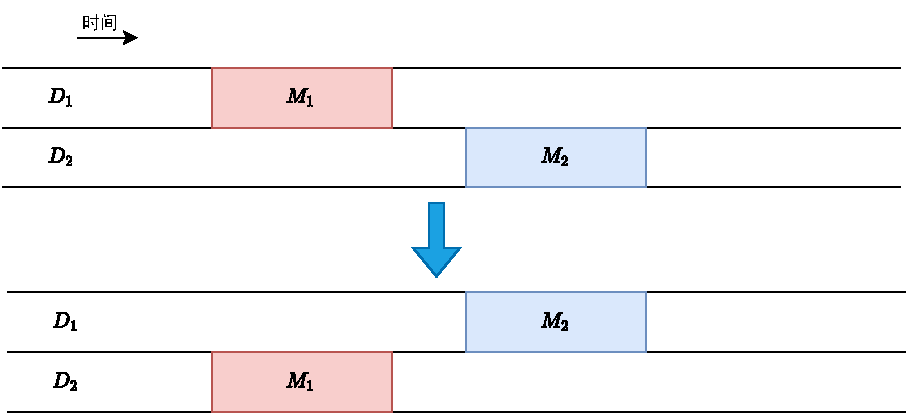
\includegraphics[width=0.7\textwidth]{images/基于边缘计算的任务资源调度算法_任务交换算子.pdf}
    \caption{任务交换邻域结构}
    \label{fig:任务交换邻域结构}
\end{figure}

第二种邻域结构为无人机间任务转移邻域结构,如图~\ref{fig:无人机间任务转移邻域结构}所示,具体操作流程如下:

\begin{enumerate}[label=(\arabic*)]
    \item {选取任务\(M_1\)、\(M_3\);}
    \item {获取用于处理任务\(M_1\)与\(M_3\)的无人机设备\(U_1\)与\(U_2\);}
    \item {将任务\(M_1\)分配给无人机设备\(U_2\)处理,即原本由无人机设备\(U_1\)处理任务\(M_1\),
    变为由无人机设备\(U_2\)处理任务\(M_1\)。}
\end{enumerate}

\begin{figure}[!htbp]
    \centering
    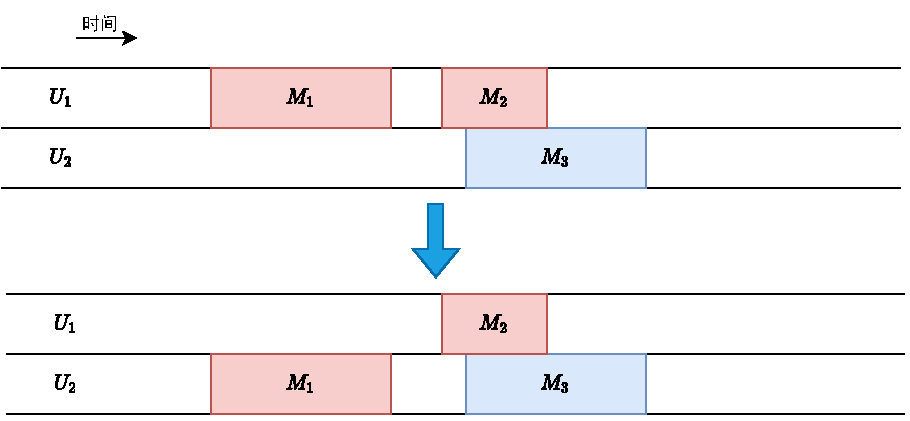
\includegraphics[width=0.7\textwidth]{images/基于边缘计算的任务资源调度算法_无人机间任务转移算子.pdf}
    \caption{无人机间任务转移邻域结构}
    \label{fig:无人机间任务转移邻域结构}
\end{figure}

第三种邻域结构为无人机向服务器转移任务邻域结构,如图~\ref{fig:无人机向服务器转移任务邻域结构}所示,具体操作流程如下:

\begin{enumerate}[label=(\arabic*)]
    \item {选取任务\(M_1\);}
    \item {获取用于处理任务\(M_1\)的无人机设备\(U\);}
    \item {将任务\(M_1\)分配给服务器设备\(C\)处理,即原本由无人机设备\(U\)处理任务\(M_1\),
    变为由服务器设备\(C\)处理任务\(M_1\)。}
\end{enumerate}

\begin{figure}[!htbp]
    \centering
    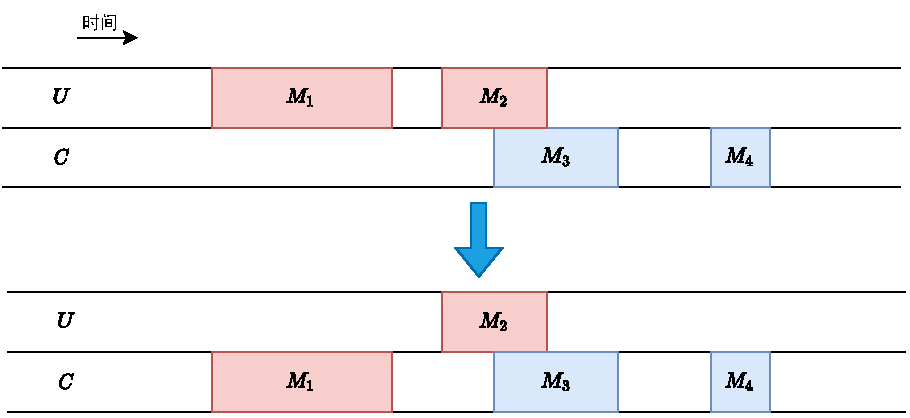
\includegraphics[width=0.7\textwidth]{images/基于边缘计算的任务资源调度算法_无人机向服务器转移任务算子.pdf}
    \caption{无人机向服务器转移任务邻域结构}
    \label{fig:无人机向服务器转移任务邻域结构}
\end{figure}

第四种邻域结构为服务器向无人机转移任务邻域结构,如图~\ref{fig:服务器向无人机转移任务邻域结构}所示,具体操作流程如下:

\begin{enumerate}[label=(\arabic*)]
    \item {选取由服务器处理的任务\(M_1\);}
    \item {获取无人机设备\(U\);}
    \item {将任务\(M_1\)分配给无人机设备\(U\)处理,即原本由服务器设备\(C\)处理任务\(M_1\),
    变为由无人机设备\(C\)处理任务\(M_1\)。}
\end{enumerate}

\begin{figure}[!htbp]
    \centering
    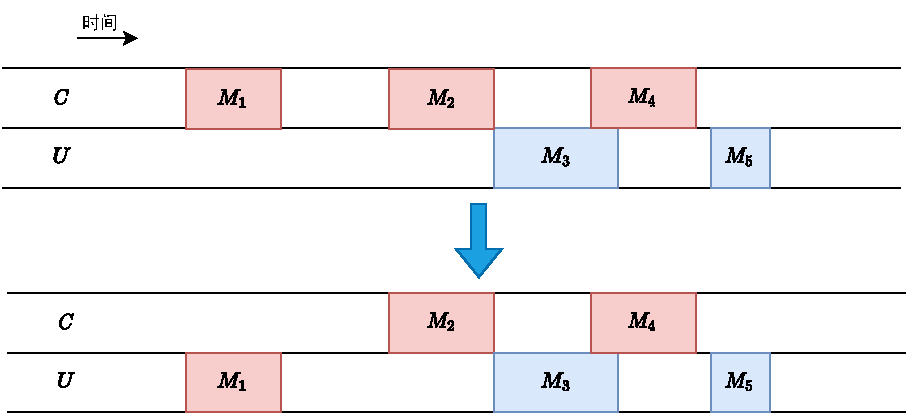
\includegraphics[width=0.7\textwidth]{images/基于边缘计算的任务资源调度算法_服务器向无人机转移任务算子.pdf}
    \caption{服务器向无人机转移任务邻域结构}
    \label{fig:服务器向无人机转移任务邻域结构}
\end{figure}

\subsubsection{自适应机制设计}

对于小节~\ref{sec:neighbor_design}中所述的邻域结构而言,在不同的情况下每个邻域结构的表现会存在差异,因此为使得算法性能更好,本文提出了基于优胜劣汰机制的邻域结构权重自适应机制,该机制能够使得表现优异的邻域结构在下次选择是被选到的机会更大,而表现较差的邻域结构则被选到的机会更小。

在算法初始化时,每个邻域结构的权重均初始化为1。在之后权重的迭代更新中,为了避免滚雪球现象,即某个邻域结构在连续非常多次表现优异后,即使此后该邻域领域的表现非常差,选择其他邻域结构也非常小,或是连续非常多次表现较差时,即使此后该邻域领域的表现非常优异,继续选择该邻域结构的概率非常小,因此在设计该机制时,本文根据生成的新解的质量与当前解的质量进行比较,此处引入\(w^r_i\)作为第\(i\)个邻域结构被第\(r\)次选中并计算完成后的权重,\(\Delta E\)为解的质量下降的值,那么有

\begin{equation}
    w^r_i = 
    \begin{aligned}
    \begin{cases}
        \bar{w^r} \quad &\text{if} \quad \Delta E > 0 \\
        0.8 \cdot w^{r-1}_i \quad &\text{if} \quad \Delta E < 0
    \end{cases} 
    \end{aligned}\nonumber
\end{equation}


另外,由于模拟退火算法在运行中会存在初期温度高,同时未达到局部最优解的情况,以及末期温度低,同时达到局部最优解的情况,导致其非更优解接受概率的利用程度不高,所以模拟退火算法的性能仍有待提高。

为提高模拟退火算法的性能,更充分地利用其跳出局部最优解的机制,此处采用了自适应温度机制取代了原有的温度机制。

此处引入\(r_{i}\)作为算法第\(i\)次运行后没有得到更优解的次数,即需要计算非更优解接受概率的次数,当直接得到了更优解时\(r_{i} = 0\),算法未运行时\(r_{0} = 0\),即

\begin{equation}
    r_i = 
    \begin{aligned} 
    \begin{cases}
        r_{i-1} + 1 \quad &\text{if} \quad \Delta E > 0\\
        r_{i-1} &\text{if} \quad \Delta E = 0 \\
        0 &\text{if} \quad \Delta E < 0
    \end{cases}
    \end{aligned}
    \nonumber
\end{equation}

同时使用迭代次数\(N\)来控制整个算法的逻辑。与模拟退火算法相比,其总的求解次数仅由\(N\)决定,而模拟退火算法的总求解次数为\(N \cdot \log_{r}\frac{T_{0}}{T_{\text{end}}}\)。

设定一个最低温度\(T_{\min}\),升温速率\(\rho\)以及温控参数\(\delta\),使得第\(i\)次计算温度\(T_{i}\)时使用如下公式:

\begin{equation}
    T_i = T_{\min} + \rho \cdot \ln (1 + \frac{r_i}{\delta})
    \nonumber
\end{equation}

如此便能够在能够寻求到最优解的情况下维持低温,在到达局部最优解、需要到达新的局部最优解时能够通过升高温度来跳出局部最优解,从而使算法具有更好的鲁棒性。

\subsection{基于FD的动态场景下的任务计算资源调度算法}

在计算资源调度的动态场景中,由于每个无人机有两种决策方式:将任务数据传输至地面端服务器,由地面端服务器进行计算;将任务数据传输至边缘端无人机,由边缘端无人机进行计算。

\begin{figure}[!htbp]
    \centering
    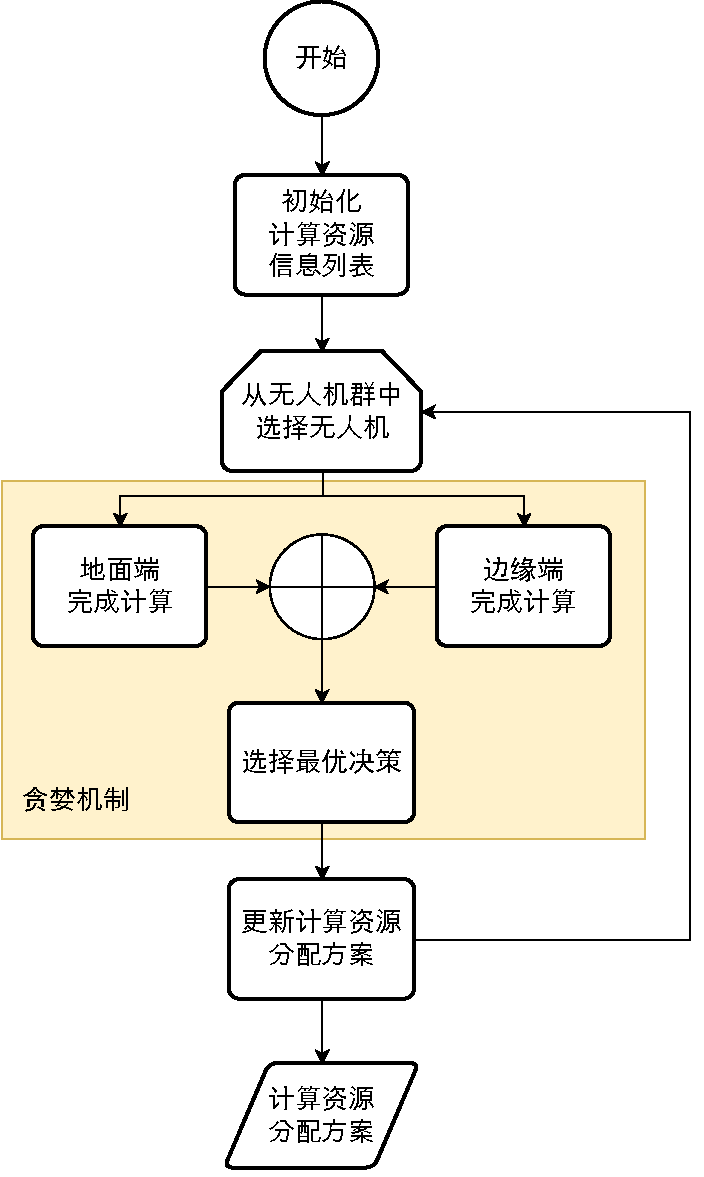
\includegraphics[width=0.6\textwidth]{./images/fd.pdf}
    \caption{FD算法流程图}
    \label{fig:FD算法流程图}
\end{figure}


因此,在满足算法生成的计算资源调度方案具有实用性的条件下,为使得算法的运行时间尽可能短,本算法在无人机决策时采用了贪婪机制(见图\ref{fig:FD算法流程图}),在对所有无人机进行遍历决策后,即可生成计算资源调度方案。

\subsection{算法流程图}

根据上述内容,本文提出的面向边缘计算的任务计算资源调度算法的运行流程如下,首先从对应数据库中获取当前的计算型侦察任务的具体信息以及无人机、服务器的计算资源的信息,在初始化算法参数后,根据以上信息生成初始解,然后进行一定次数的迭代;在每步迭代中,算法从任务交换邻域结构、无人机间任务转移邻域结构、无人机向服务器转移任务邻域结构、服务器向无人机转移任务邻域结构中选择一个进行当前解的邻域变动,得到优化结果,判断该优化结果与目前的最优解是否更优,若更优则保存,否则进行概率判断,按随机概率确定是否保存,保存则更新最优解,然后更新算法参数,直至迭代结束,在迭代结束后,即可得到当前任务的计算资源最优分配方案。总流程如图~\ref{fig:基于边缘计算的任务资源调度算法流程图}所示。

\begin{figure}[!htbp]
    \centering
    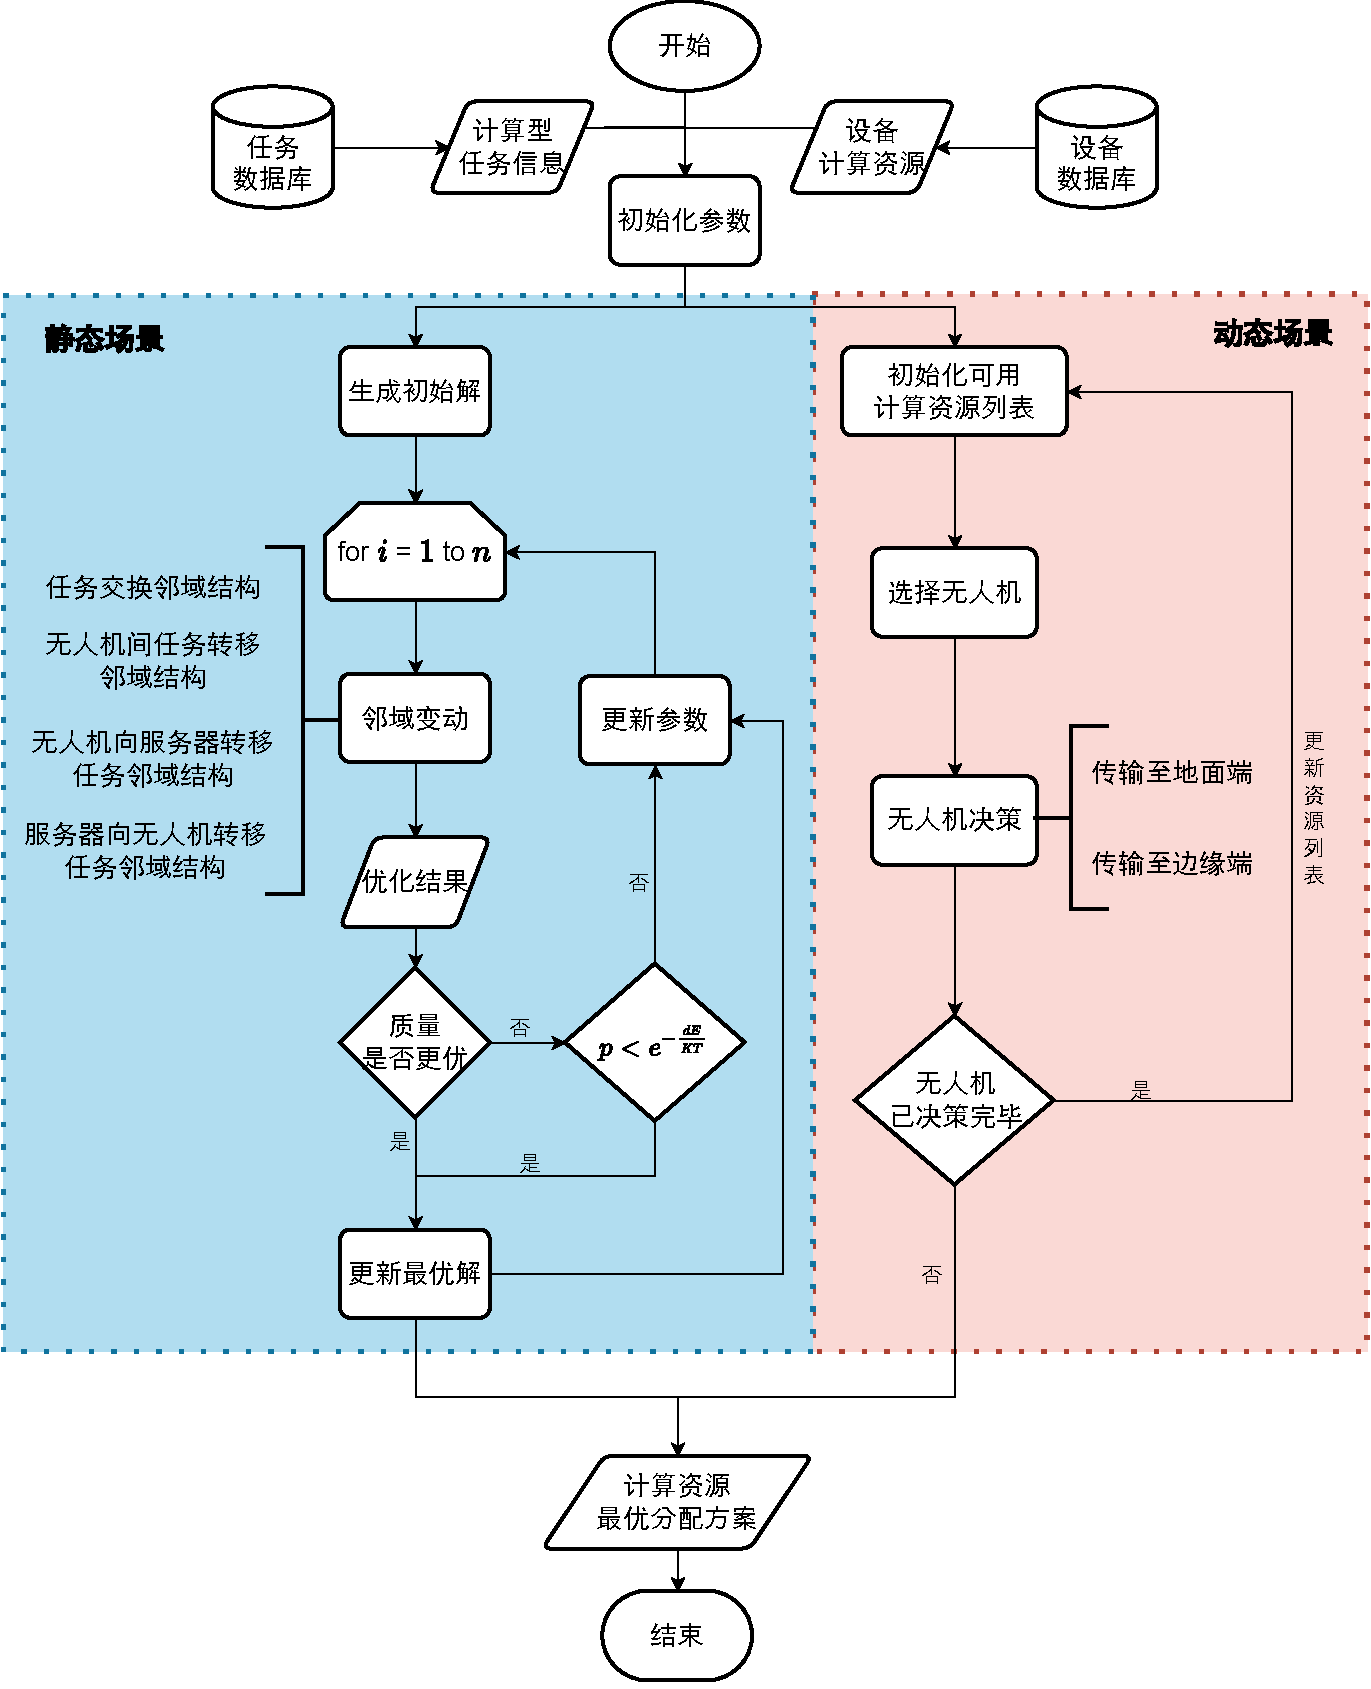
\includegraphics[width=\textwidth]{images/基于边缘计算的任务资源调度算法流程图.pdf}
    \caption{面向边缘计算的任务计算资源调度算法流程图}
    \label{fig:基于边缘计算的任务资源调度算法流程图}
\end{figure}

